\newif\ifvimbug
\vimbugfalse

\ifvimbug
\begin{document}
\fi

\exercise{Non-parametric Density Estimation}
 
In this exercise, you will use the datasets \texttt{nonParamTrain.txt} for training and \texttt{nonParamTest.txt} for evaluating the performance of your model.

\begin{questions}

%----------------------------------------------

\begin{question}{Histogram}{4}
Compute and plot the histograms using $0.02$, $0.5$, $2.0$ size bins of the training data.  
Intuitively, indicate which bin size performs the best and explain why. Knowing only these three trials, would you be sure that the one you picked is truly the best one? Attach the plot of the histograms and a snippet of your code.

\begin{answer}
The first figure \ref{fig:histogram1} shows a Histogram of the data with bin size 0.02. The "spicky" behavior and empty bins which are conssistend throughout the Histogram, indicate that the bin size has been chosen to to small (to much Variance).	

In the next Figure \ref{fig:histogram2} you can imagine a trend for the underlying distribution. This indicates a good bin size.


The third histogram \ref{fig:histogram3} also schows a trend of the underlying function, but compared to figure \ref{fig:histogram2} some of details get lost in the representation. Meaning that the bin size has been choosen to big (to much Bias).

Bonus: This last histogram \ref{fig:histogram4} is an histogram with the number of bins determined by Sturges Rule. It's shape is similiar to figure (2), only beeing a bit more smooth. However Sturges rule is critized to smooth the Histogram to much (Hyndman, 1995) and should be only used as a rule of thumb. In this case it adds futher believe into a bin size of about 0.5

However in the end for these four bin sizes, we cant be completly sure that the one choose is the best, but we have atleast good evidence for it.
	
\end{answer}
\end{question}


\begin{figure}[H]
	\centering
	\begin{subfigure}[b]{0.4\linewidth}
		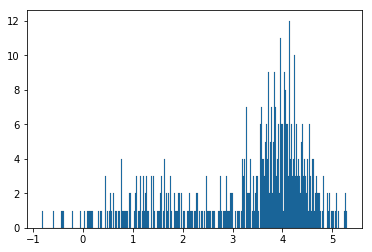
\includegraphics[width=\linewidth]{pictures/histogram002.png}
		\caption{Bin Size 0.02.}
		\label{fig:histogram1}
	\end{subfigure}
	\begin{subfigure}[b]{0.4\linewidth}
		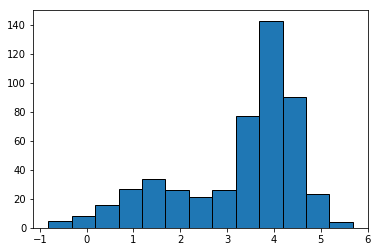
\includegraphics[width=\linewidth]{pictures/histogram05.png}
		\caption{Bin Size 0.5.}
		\label{fig:histogram2}
	\end{subfigure}
	\caption{First two Histograms}
\end{figure}

\begin{figure}[H]
	\centering
	\begin{subfigure}[b]{0.4\linewidth}
		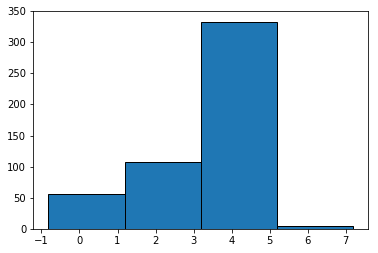
\includegraphics[width=\linewidth]{pictures/histogram2.png}
		\caption{Bin Size 2}
		\label{fig:histogram3}
	\end{subfigure}
	\begin{subfigure}[b]{0.4\linewidth}
		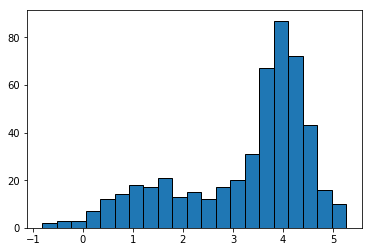
\includegraphics[width=\linewidth]{pictures/histogramSturge.png}
		\caption{Bin size calculated with Sturges Rule.}
		\label{fig:histogram4}
	\end{subfigure}
	\caption{Last two Histograms}	
\end{figure}

	
Snippet of the code used: 
\begin{lstlisting}{}
import numpy as np
train = np.loadtxt("nonParamTrain.txt");

import matplotlib.pyplot as plt
binwidth = 0.02
bin_sequence = np.arange(min(train), max(train) + binwidth, binwidth)  
plt.hist(train, bins=bin_sequence, edgecolor="black" ,linewidth=0.1);
\end{lstlisting}

%----------------------------------------------

\begin{question}{Kernel Density Estimate}{6}
Compute the probability density estimate using a Gaussian kernel with $\sigma=0.03$, $\sigma=0.2$ and $\sigma=0.8$ of the training data. Compute the log-likelihood of the data for each case, compare them and show which parameter performs the best.
Generate a single plot with the different density estimates and attach it to your solutions. Plot the densities in the interval $x \in [-4,8]$, attach a snippet of your code and comment the results.

\begin{answer}
The log-likelihood for the first Gaussian kernel with $\sigma = 0.03$ is: $-674.7$. 

The log-likelihood for the second Gaussian kernel with $\sigma = 0.2$ is: $-717.0$. 

The log-likelihood for the third Gaussian kernel with $\sigma = 0.08$ is: $-795.7$. 

From campring the log-likelihoods the first kernel should be the best one. But by futher observing the graphs it seems that the second kernel is the best suited for the task.
\end{answer}
\end{question}

\begin{figure}[!h]
	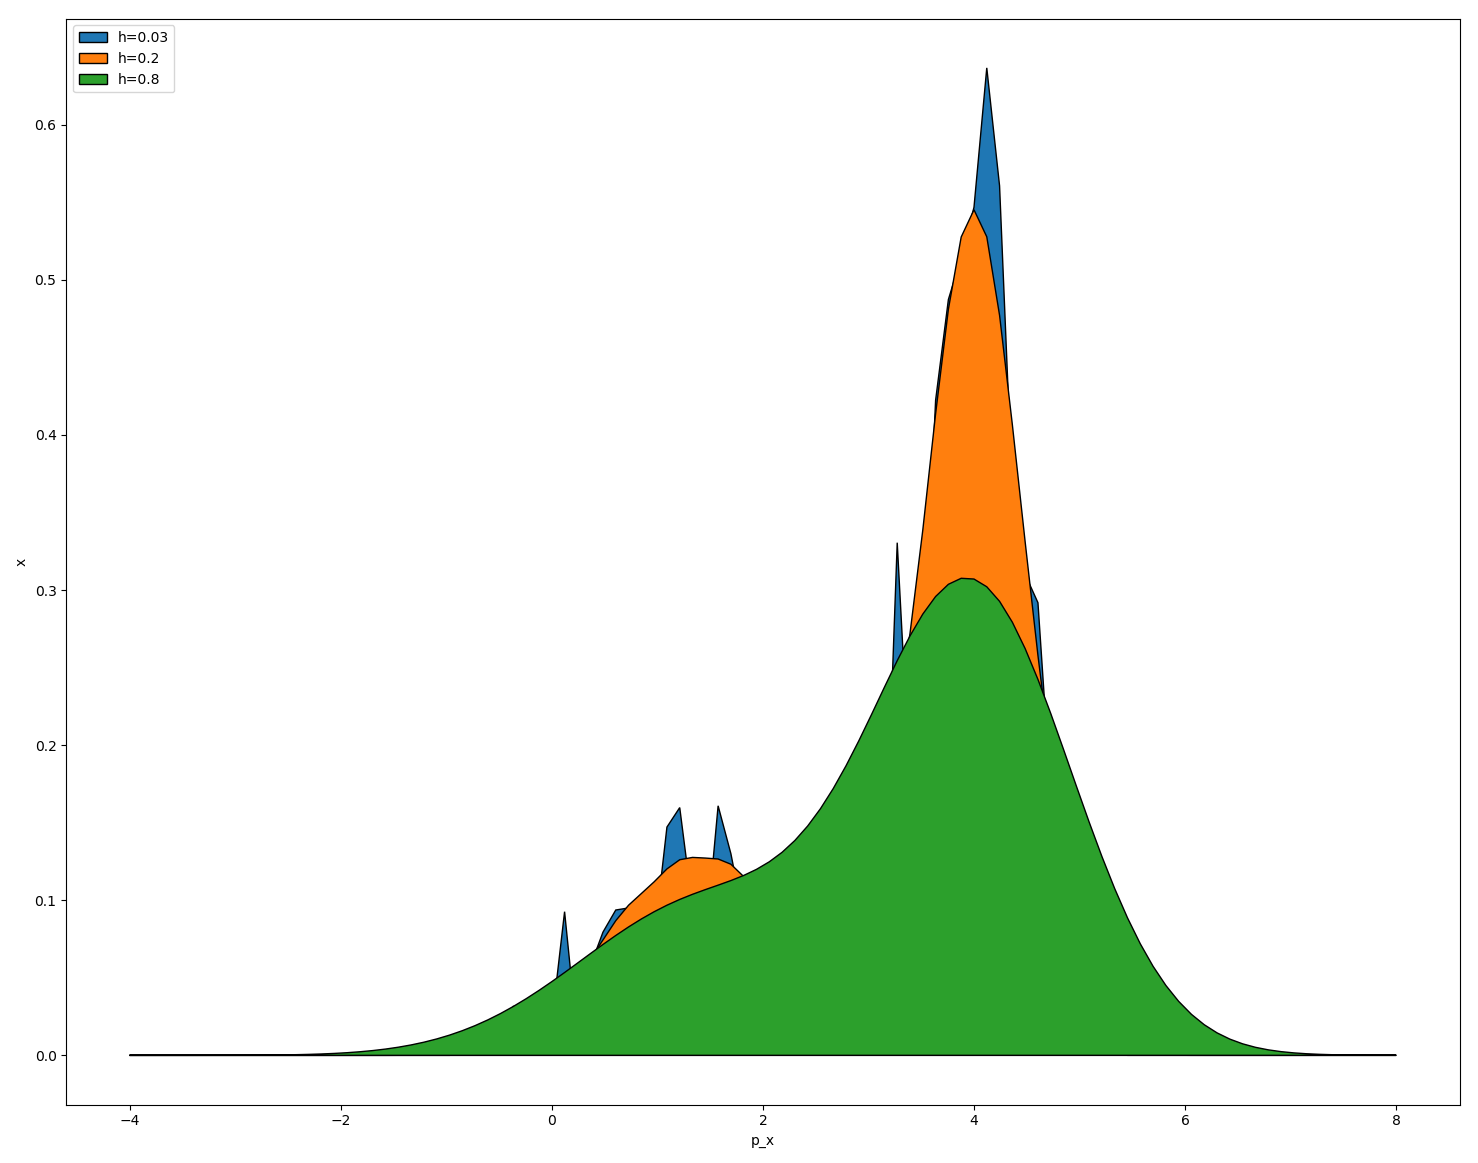
\includegraphics[width=0.8\linewidth]{pictures/kdplot.png}
	\centering
	\label{kd}
	\caption{Kernel density estimation for $\sigma = h = [0.03, 0.2, 0.8]$}
\end{figure}

\begin{figure}[H]
	\centering
	\begin{subfigure}[b]{0.3\linewidth}
		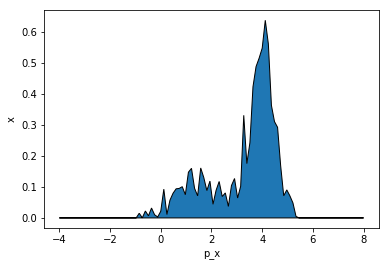
\includegraphics[width=\linewidth]{pictures/kd003.png}
		\caption{Kernel Size of 0.03}
		\label{fig:kd003}
	\end{subfigure}
	\begin{subfigure}[b]{0.3\linewidth}
		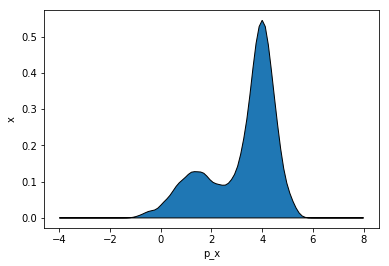
\includegraphics[width=\linewidth]{pictures/kd02.png}
		\caption{Kernel Size of 0.2.}
		\label{fig:kd02}
	\end{subfigure}
	\begin{subfigure}[b]{0.3\linewidth}
	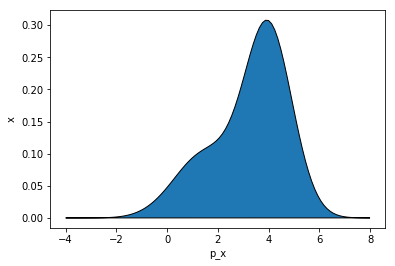
\includegraphics[width=\linewidth]{pictures/kd08.png}
	\caption{Kernel Size of 0.8.}
	\label{fig:kd03}
\end{subfigure}
	\caption{All the plots seperated}
\end{figure}


Snippet of the code used: 
\begin{lstlisting}{}
def gaussian(x,h):
    return np.exp(-x**2/(2*h**2))/(h*np.sqrt(2*np.pi))  

N = train.size
X_plot = np.linspace(-4, 8, 100)
sum1 = np.zeros(len(X_plot))
sum2 = np.zeros(len(X_plot))
sum3 = np.zeros(len(X_plot))

for i in range(0, N):
    sum1 += ((gaussian(X_plot - train[i], h=0.03)) / N)

# Plot the result
plt.fill(X_plot, sum1, edgecolor="black" ,linewidth=1)
plt.xlabel("p_x")
plt.ylabel("x")

# Calculate the likelihood
likelihood_sum = 0
for i in range(0, N):
    likelihood = 0
    for j in range(0, N):
        likelihood += ((gaussian(train[i] -train[j], h=0.03)) / N)
    likelihood = math.log(likelihood)
    likelihood_sum += likelihood
print(likelihood_sum)
\end{lstlisting}

%----------------------------------------------

\begin{question}{K-Nearest Neighbors}{6}
Estimate the probability density with the K-nearest neighbors method with $K=2, K=8, K=35$.
Generate a single plot with the different density estimates and attach it to your solutions. Plot the densities in the interval $x \in [-4,8]$, attach a snippet of your code and comment the results.

\begin{answer}


\end{answer}

\end{question}


\begin{figure}[!h]
	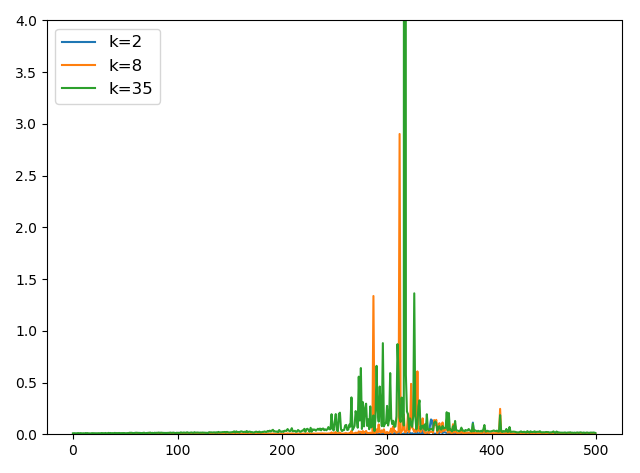
\includegraphics[width=0.62\linewidth]{pictures/knnplot.png}
	\centering
	\label{kd}
	\caption{K-Nearest Neighbors for $k=2, k=8, k=35$}
\end{figure}

\begin{lstlisting}{}
import numpy as np
import matplotlib.pyplot as plt
import math

train = np.loadtxt("nonParamTrain.txt");
k = 35
N = train.size
distances = np.zeros([N, N - 1])
pd = np.zeros(N)
x_axis = np.linspace(-4, 8, N)

# plot density
for i in range(0, N):
    for ii in range(0, N - 1, ):
        distances[i][ii] = abs(train[i] - train[ii])

    distances[i, :] = np.sort(distances[i, :]);
    pd[i] = distances[i][-k]  # k nearest neighbor

result = k / (N * abs(x_axis - pd))
plt.plot(result)

# Compute log likelihood
distances = np.zeros([N, N - 1])
pd = np.zeros(N)
for i in range(0, N):
    for ii in range(0, N - 1, ):
        distances[i][ii] = abs(train[i] - train[ii])

    distances[i, :] = np.sort(distances[i, :]);
    pd[i] = distances[i][-k]  # k nearest neighbor

likelihood = 0
for i in range(0, N):
    likelihood += math.log(k / (N * abs(train[i] - pd[i])))
print(likelihood)
\end{lstlisting}

%----------------------------------------------

\begin{question}{Comparison of the Non-Parametric Methods}{4}
Estimate the log-likelihood of the testing data using the KDE estimators and the K-NN estimators.
Why do we need to test them on a different data set? Compare the log-likelihoods of the estimators w.r.t. both the training and testing sets in a table. Which estimator would you choose?

\begin{answer}
The following table lists all results for the log-likelihoods of the estimators w.r.t both the training and testing sets in a table. The First three rows are for the training set with $\sigma = [0.03, 0.2, 0.8]$ and $k = [2, 8, 35]$ and the next three for the test set using the same order oder paramterization.

Actually from the log-likelihoods it seems that all estimators perform badly. However the Kernel Density Estimate using Gaussian kernel has much better results than the knn-Algorithm so its prefferable.


\begin{center}
	\begin{tabular}{c| c | c  }
		& KDE & KNN \\
		\hline 
		1. & -675 & -2675 \\
		2. & -717 & -875 \\
		3. & -795 & -1273 \\
		\hline		
		4. & -2812 & -14631 \\
		5. & -2877 & -11115 \\
		6. & 3192 & -4469
	\end{tabular}
\end{center}

\end{answer}

\end{question}



\end{questions}
